% Lintai Bao's hardware operations-manual report style.
\documentclass[lang=en,11pt,a4paper,bibend=bibtex]{elegantpaper}
\usepackage{xeCJK}
\setCJKmainfont{FandolSong-Regular.otf}
\setCJKsansfont{FandolSong-Regular.otf}
\setCJKmonofont{FandolSong-Regular.otf}
\usepackage{tikz,pgfplots,tabularx,titlesec,fancyhdr}
\usetikzlibrary{arrows.meta,positioning,calc}
\pgfplotsset{compat=1.18}
\geometry{left=23mm,right=23mm,top=21mm,bottom=22mm,headheight=15pt,headsep=7mm}
\linespread{1.10}
\setlength{\parindent}{0pt}
\setlength{\parskip}{5pt}
\setlength{\emergencystretch}{2em}
\definecolor{accent}{HTML}{234D64}
\definecolor{muted}{HTML}{59646C}
\definecolor{light}{HTML}{F0F4F6}
\hypersetup{colorlinks=true,linkcolor=accent,urlcolor=accent}
\titleformat{\section}{\Large\sffamily\bfseries\color{accent}}{\thesection}{0.6em}{}
\titleformat{\subsection}{\normalsize\sffamily\bfseries}{\thesubsection}{0.6em}{}
\titlespacing*{\section}{0pt}{9pt}{8pt}
\titlespacing*{\subsection}{0pt}{8pt}{3pt}
\pagestyle{fancy}
\fancyhf{}
\fancyhead[L]{\small\sffamily\color{muted}EXPERIMENT 2\enspace /\enspace ROBOMASTER EP}
\fancyhead[R]{\small\sffamily\color{muted}\studentname}
\fancyfoot[L]{\small\sffamily\color{muted}\studentid\quad\textbullet\quad Individual laboratory report}
\fancyfoot[R]{\small\sffamily\thepage}
\renewcommand{\headrulewidth}{0.3pt}
\renewcommand{\footrulewidth}{0pt}
\captionsetup{font=small,labelfont=bf,labelsep=period,skip=5pt,hypcap=false}
\renewcommand{\arraystretch}{1.18}
\newcolumntype{Y}{>{\raggedright\arraybackslash}X}
\newcommand{\code}[1]{{\small\nolinkurl{#1}}}
\newcommand{\source}[1]{{\small\color{muted}Source: #1}\par}
\newcommand{\reportnote}[1]{\par\smallskip\noindent\colorbox{light}{\parbox{\dimexpr\linewidth-2\fboxsep}{\small #1}}\par\smallskip}
\newcommand{\reporttitle}[1]{\vspace*{2mm}{\small\sffamily\bfseries\color{accent}FIXED-POINT PICK-AND-PLACE}\par\vspace{2mm}{\LARGE\sffamily\bfseries #1\par}\vspace{3mm}{\large\studentname\enspace\studentcn}\par{\small Student ID: \studentid\quad |\quad Individual report}\par\vspace{3mm}\hrule\vspace{3mm}}
\tikzset{box/.style={draw=accent,fill=light,rounded corners=2pt,align=center,font=\small,minimum height=9mm},arr/.style={-{Latex[length=2mm]},thick,draw=accent}}
\newcommand{\teamtable}{%
\par\smallskip
\begingroup\small\renewcommand{\arraystretch}{1.08}
\begin{tabularx}{\linewidth}{@{}>{\raggedright\arraybackslash}p{25mm}>{\raggedright\arraybackslash}p{21mm}Y@{}}\toprule
Member & Work area & Main responsibility \\\midrule
Ning Bo & Simulation & Set up the environment and scene; load models and launch the simulation.\\
Huang Junbiao & Simulation & Work on the motion program and debug grasping, transfer and repeated cycles.\\
Qi Yongyue & Simulation results & Organize logs, analyse results and prepare report material.\\
Bao Lintai & Hardware & SDK communication, task sequence, chassis turn/return and exception handling; joint trials.\\
Xue Yutong & Hardware & Pick/release waypoints, approach/lift heights, gripper adjustment and retention checks; joint trials.\\\bottomrule
\end{tabularx}\par\endgroup}
\newcommand{\commonrequirements}{%
\section{Experiment requirements and individual scope}
The experiment develops a fixed-point grasping task without visual localization: home, approach A, descend, grip, lift, transfer to B, release and return. The course requires a complete simulation launch, state publication, saved trajectories/results/errors, joint and reachability checks, and at least four successful transfers in five consecutive trials. Hardware verification additionally requires supervised low-speed operation, safe failure handling and individual safety-operation checks [1].

Because of equipment availability, our group used the DJI RoboMaster EP arm and gripper instead of the specified mechArm 270. The simulation uses ROS 2 Humble, Gazebo Fortress and custom kinematics/control on a Jetson Linux system. The physical implementation uses the RoboMaster Python SDK. This is a platform adaptation, not an unchanged ROS 2 hardware backend.
}
\newcommand{\commonlimits}{%
\reportnote{Scope of evidence. Simulation repeats A$\rightarrow$B and verifies home after every cycle; the object is reset only between cycles. Hardware alternates A/B, pauses for human grasp confirmation and returns home after all five cycles. Shared ROS 2 interfaces, parameter-only hardware switching and each member's safety check are not demonstrated by the supplied records.}}
\newcommand{\mainresults}{%
\begin{center}\small
\begin{tabular}{@{}crrrcc@{}}\toprule
Cycle & Error (mm) & Heading ($^\circ$) & Time (s) & Placed & Home \\\midrule
1 & 2.274 & 0.445 & 67.01 & Yes & Yes\\
2 & 5.604 & 0.329 & 59.72 & Yes & Yes\\
3 & 4.192 & 0.404 & 60.92 & Yes & Yes\\
4 & 4.577 & 0.459 & 61.09 & Yes & Yes\\
5 & 5.144 & 0.405 & 61.29 & Yes & Yes\\\bottomrule
\end{tabular}
\end{center}
\source{Recorded simulation run \code{20260913_153855_682865/results.json}; error is horizontal distance from configured B, heading is absolute home-heading error.}}
\newcommand{\hardwareresult}{%
\subsection{Physical validation: team-observed outcome}
The team confirmed that all five hardware transfers succeeded with no observed abnormalities. Cycles 1, 3 and 5 moved A$\rightarrow$B; cycles 2 and 4 moved B$\rightarrow$A. Each lift was followed by a fresh human \code{y} confirmation before rotation; final heading restoration and homing followed cycle 5. This is an observed 5/5 result, not an instrumented precision or timing measurement. No real-hardware position-error, duration or force data are available, and five successes do not establish long-run reliability.}
\newcommand{\githubsection}{%
\clearpage
\section{Shared GitHub repository and commit evidence}
The complete group archive is stored in the
\href{https://github.com/ccx8kg5qpd-debug/robomaster-ep-fixed-point-grasping}
{shared public GitHub repository}. The repository address is
\nolinkurl{github.com/ccx8kg5qpd-debug/robomaster-ep-fixed-point-grasping}.
It contains the simulation and hardware programs, model resources, saved results,
the complete simulation recording and all five individual report sources.

\begin{center}
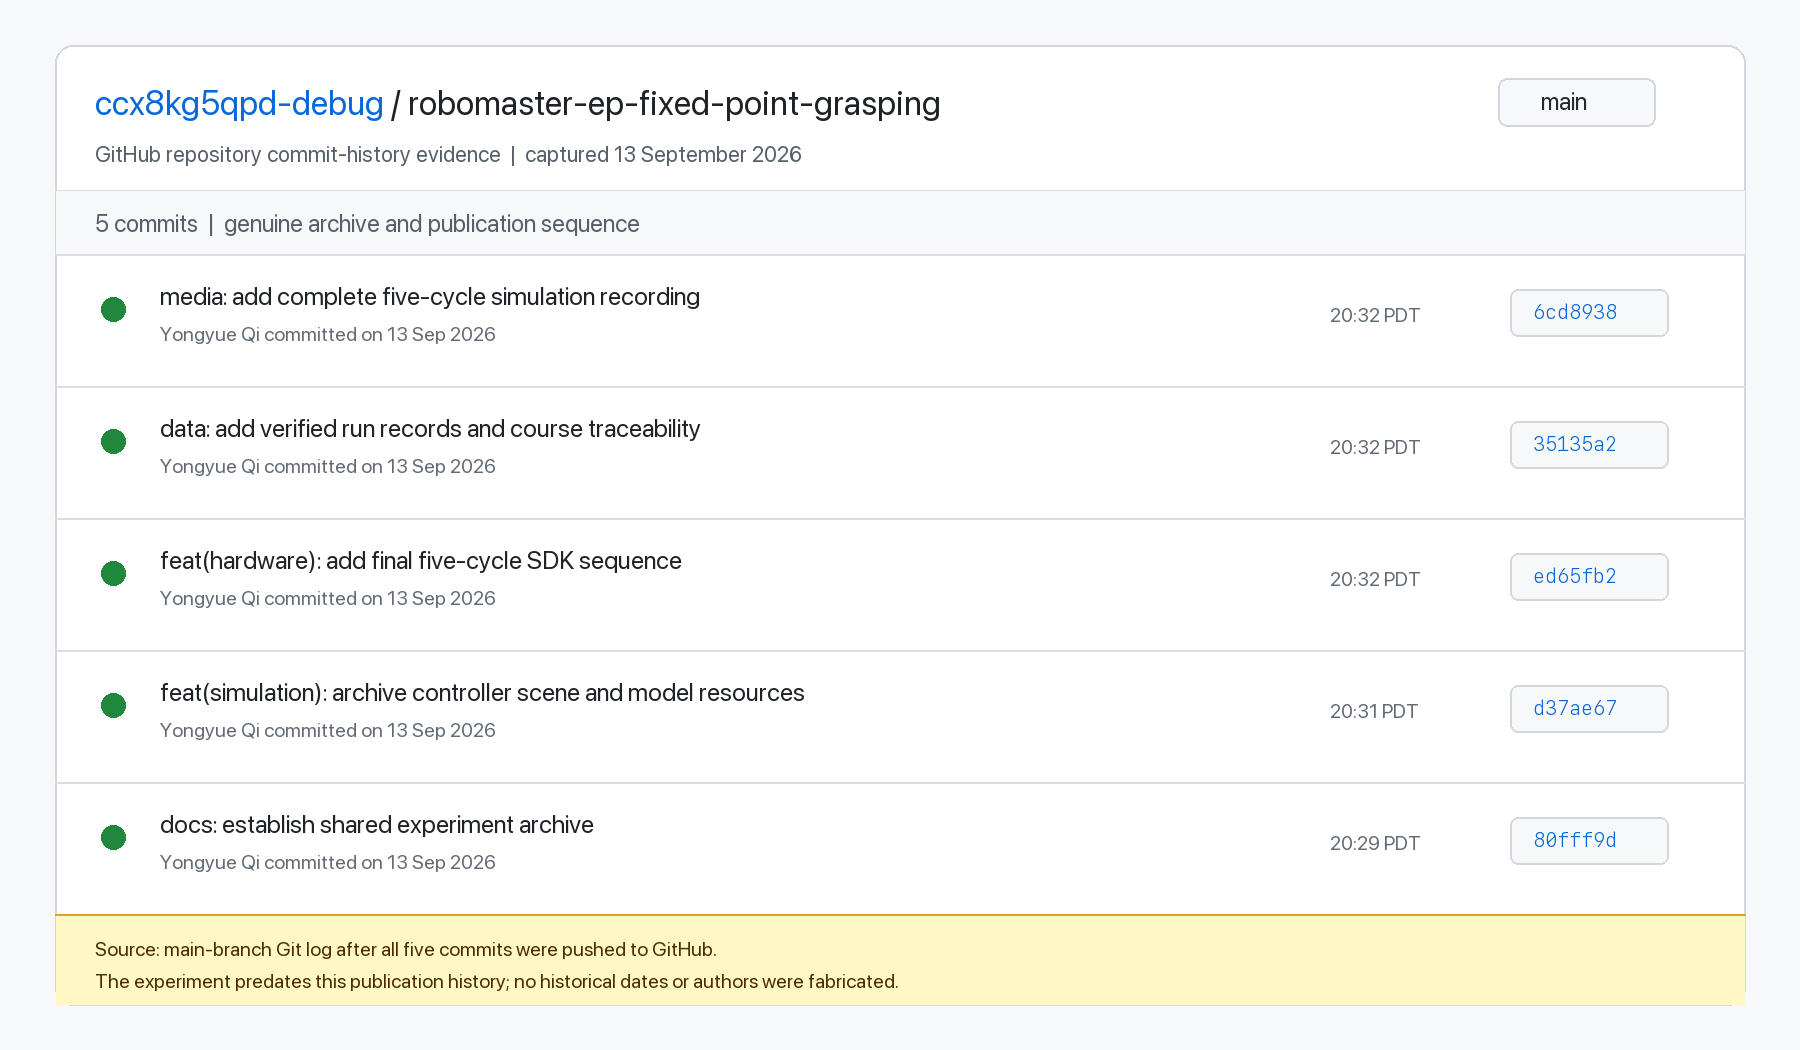
\includegraphics[width=\linewidth]{assets/commit_history_snapshot.png}
\captionof{figure}{Commit-history evidence captured after the first five project
materials commits had been pushed to the shared GitHub repository.}
\end{center}

\reportnote{Traceability note. The experiment was completed before the GitHub
repository was assembled. These genuine commits document the later review,
organization and publication sequence; they are not presented as a fabricated
contemporaneous development history. The screenshot records the five commits
visible at capture time, before this revised report was added.}
}
\newcommand{\referencesblock}{%
\section*{Sources and traceability}
{\footnotesize
[1] Course handout, \emph{Fixed-Point Robotic-Arm Grasping: Simulation Development and Hardware Validation}, S16--S20 / E5; individual-report assignment requirements.\par
[2] Shared team repository, \href{https://github.com/ccx8kg5qpd-debug/robomaster-ep-fixed-point-grasping}{robomaster-ep-fixed-point-grasping}, assembled 13 September 2026: simulation source/configuration, \code{real_v2_five_cycles_manual.py}, saved logs and reports. Primary numerical record: \code{20260913_153855_682865}.\par
[3] Team conversation fact-check materials, 13 September 2026, for development history; subsequent team confirmation for the completed five-cycle hardware run. Historical failures are not counted as final-run failures.\par
[4] Community model resources: \href{https://github.com/jeguzzi/robomaster_ros}{jeguzzi/robomaster\_ros}, archived commit \code{c05a39d7f0fa}. Report layout uses \href{https://ctan.org/pkg/elegantpaper}{ElegantPaper}, distributed under LPPL 1.3c.
}}

\definecolor{accent}{HTML}{163A5F}
\definecolor{muted}{HTML}{5C6670}
\definecolor{light}{HTML}{EEF2F5}
\definecolor{signal}{HTML}{E87824}
\geometry{left=20mm,right=20mm,top=24mm,bottom=20mm,headheight=16pt,headsep=6mm}
\hypersetup{linkcolor=signal,urlcolor=signal}
\titleformat{\section}{\Large\sffamily\bfseries\color{accent}}{\colorbox{signal}{\textcolor{white}{\thesection}}}{0.7em}{}
\titleformat{\subsection}{\normalsize\sffamily\bfseries\color{signal}}{\thesubsection}{0.55em}{}
\fancyhead[L]{\small\sffamily\bfseries\color{accent}ROBOMASTER EP / OPERATIONS MANUAL}
\fancyhead[R]{\small\sffamily\color{muted}\studentid}
\fancyfoot[L]{\scriptsize\sffamily\color{muted}SDK sequence, chassis motion and exception handling}
\fancyfoot[R]{\small\sffamily\bfseries\color{signal}\thepage}
\renewcommand{\headrulewidth}{1.1pt}
\renewcommand{\reportnote}[1]{\par\smallskip\noindent\fcolorbox{signal}{light}{\parbox{\dimexpr\linewidth-2\fboxsep-2\fboxrule}{\small\textcolor{signal}{\textbf{OPERATION NOTE}}\quad #1}}\par\smallskip}
\renewcommand{\reporttitle}[1]{\vspace*{1mm}\noindent\colorbox{accent}{\parbox{\dimexpr\linewidth-2\fboxsep}{\color{white}\sffamily\bfseries EXPERIMENT 02 / OPERATIONS MANUAL}}\par\vspace{5mm}{\fontsize{21}{25}\selectfont\sffamily\bfseries\color{accent}#1\par}\vspace{4mm}{\large\sffamily\studentname\enspace\studentcn\par}{\small Student ID: \studentid\quad|\quad Individual operations-manual design}\par\vspace{4mm}{\color{signal}\rule{\linewidth}{1.6pt}}}

\newcommand{\studentname}{Bao Lintai}
\newcommand{\studentcn}{包林泰}
\newcommand{\studentid}{24020036004}
\begin{document}
\reporttitle{Hardware Program Execution\\and Test Procedure}
\commonrequirements
\subsection{My responsibility and team interfaces}
Xue Yutong and I share the hardware experiment and integrated trials. My main responsibility is SDK communication, motion sequencing, chassis turning and return, and exception handling. Xue's main responsibility is the pick/release waypoints, approach/lift heights and gripper-retention adjustment. We share physical setup, parameter review and five-cycle testing. Ning Bo and Huang Junbiao handle simulation, while Qi Yongyue organizes the results. My report focuses on the whole-program execution; Xue's focuses on the arm--object interaction and its settings.
\teamtable
\commonlimits
\clearpage
\section{Hardware implementation and coordinate mapping}
\subsection{Device-specific execution}
The final physical script is \code{real_v2_five_cycles_manual.py}. It initializes a RoboMaster robot in AP connection mode and uses direct SDK arm, gripper and chassis operations. It does not call the simulation's ROS 2 task services. The team confirmed that this manual-confirmation workflow was used for the successful physical trials.
The script must run from an interactive terminal: it checks that standard input is a terminal and later waits for a new typed confirmation. Running it through a pipe would not reproduce the intended operator interaction. This is a practical execution requirement, not a change to the grasping algorithm.
\begin{center}
\begin{tabular}{@{}lrrl@{}}\toprule
SDK waypoint & $x$ (mm) & $y$ (mm) & Role\\\midrule
HOME & 82 & 80 & Retracted high position\\
HIGH & 191 & 80 & Extended high position\\
HOVER & 191 & $-1$ & Above grasp/release level\\
GRASP & 191 & $-51$ & Low pick/release position\\\bottomrule
\end{tabular}
\end{center}
The second SDK arm coordinate controls vertical position in this script. These pairs are device coordinates in millimetres, not the simulation's world $(x,y,z)$ points. HOVER is 50 mm above GRASP. Converting metres to millimetres alone cannot transform a Gazebo fingertip target into an equivalent hardware waypoint because the reference origin and mechanism representation differ.
\subsection{Initialization and transfer motion}
The script stops the wheels, opens the gripper with power setting 30, waits 1.5 s and pauses the gripper. Initial motion passes through HOME, HIGH and HOVER. Each cycle then descends to GRASP, closes with power setting 100 for 3 s and pauses, before lifting back to HOVER. These are SDK power settings and timed actions, not measurements of applied fingertip force.

After a valid human confirmation, the base turns $+32^\circ$ on odd cycles and $-32^\circ$ on even cycles, with commanded yaw speed $12^\circ$/s. The script waits for the turn action with a 15 s timeout, lowers, opens the gripper, waits and retreats to HOVER. Ordinary arm-action waits use a 12 s timeout. The task counter increments after the release/retreat sequence.
\subsection{Final return differs from simulation}
Hardware alternates A$\rightarrow$B and B$\rightarrow$A without automatic object refill. After cycle 5, it compensates the remaining heading and returns through HIGH to HOME. It does not perform the simulation's full heading-and-arm return after each individual transfer. This distinction is a factual feature of the final script, not an assumption about the recording.
\clearpage
\section{Confirmation checkpoint and stopping logic}
\subsection{Preventing transfer with an uncertain grasp}
After the 50 mm lift, the script stops base motion and clears previously buffered terminal input. It then waits up to 30 s for a fresh \code{y}. Clearing old input matters: a key pressed before seeing the lifted object should not count as a new confirmation. The human observer judges whether the cube has actually been retained before any transfer rotation is permitted.
For an individual trial, one hardware member handles controls while the other watches the object and working area. Both participate in tuning and integrated testing rather than holding permanent operator/helper roles. The checkpoint joins Xue's retention checks to my transfer logic: rotation should not begin before the current grasp has been clearly confirmed.
\begin{center}
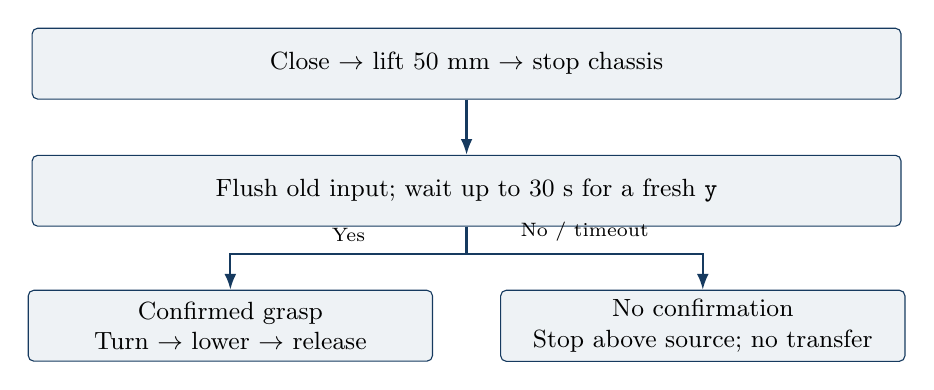
\begin{tikzpicture}[node distance=7mm]
\node[box,text width=108mm] (lift) {Close $\rightarrow$ lift 50 mm $\rightarrow$ stop chassis};
\node[box,text width=108mm,below=of lift] (check) {Flush old input; wait up to 30 s for a fresh \texttt{y}};
\node[box,text width=49mm,below=8mm of check,xshift=-30mm] (yes) {Confirmed grasp\\Turn $\rightarrow$ lower $\rightarrow$ release};
\node[box,text width=49mm,below=8mm of check,xshift=30mm] (no) {No confirmation\\Stop above source; no transfer};
\draw[arr](lift)--(check);
\draw[arr](check.south)--++(0,-.35)-|(yes.north);
\draw[arr](check.south)--++(0,-.35)-|(no.north);
\node[above=1pt,font=\scriptsize] at ($(check.south)+(-15mm,-3.5mm)$) {Yes};
\node[above=1pt,font=\scriptsize] at ($(check.south)+(15mm,-3.5mm)$) {No / timeout};
\end{tikzpicture}
\captionof{figure}{The hardware checkpoint uses operator observation, not automatic object sensing.}
\end{center}
If confirmation is absent, the script does not rotate or automatically home. It stops above the source and returns through cleanup. This avoids adding a return trajectory when object retention is uncertain. The \code{finally} block pauses gripper drive, commands zero wheel speed and closes the SDK connection.
\subsection{What the cleanup does not guarantee}
The script's cleanup is a software response, not a certified emergency-stop circuit. It does not explicitly cancel every potentially active arm action. Communication loss may also limit command delivery. Therefore, the report should not claim that the script guarantees an immediate complete mechanical stop under every failure. A physical stop/power-off provision and an attentive observer remain necessary.
\subsection{Operating procedure versus recorded evidence}
The course calls for checks of mounting, power, connections, gripper and emergency-stop arrangements, supervised low-speed first operation, and individual safety-operation checks. Those are required procedures. The supplied materials and team confirmation establish the nominal five-cycle outcome, but do not document each person's check or a final fault-injection campaign. They must not be retrospectively marked as passed solely because no abnormality was observed.
\clearpage
\section{Hardware outcome and simulation comparison}
\begin{center}
\begin{tabular}{@{}cllll@{}}\toprule
Cycle & Direction & Lift confirmation & Transfer result & Abnormality\\\midrule
1 & A$\rightarrow$B & Confirmed & Successful & None observed\\
2 & B$\rightarrow$A & Confirmed & Successful & None observed\\
3 & A$\rightarrow$B & Confirmed & Successful & None observed\\
4 & B$\rightarrow$A & Confirmed & Successful & None observed\\
5 & A$\rightarrow$B & Confirmed & Successful & None observed\\\bottomrule
\end{tabular}
\end{center}
\source{Team confirmation of five successful trials and use of the final manual-confirmation workflow; this table is not a machine-generated hardware log.}
The observed hardware success rate was 5/5, meeting the handout's at-least-4/5 transfer criterion for this sample. No measured physical placement errors, motion durations or gripping forces were supplied. Consequently, no numerical hardware precision or speed comparison is claimed.
\begin{center}\small
\begin{tabularx}{\linewidth}{@{}p{30mm}YY@{}}\toprule
Aspect & Final simulation & Final hardware\\\midrule
Control route & ROS 2, bridge and Gazebo plugins & Direct RoboMaster SDK\\
Direction & A$\rightarrow$B every cycle & Alternating A/B\\
Grasp decision & Bilateral contact and object height & Human confirmation after lift\\
Return home & Verified every cycle & At initialization and after cycle 5\\
Replenishment & Home-gated object reset, four times & No automated refill\\
Evidence & Coordinates, events and trajectory & Team-observed five successes\\\bottomrule
\end{tabularx}
\end{center}
For quantitative context, the recording-associated simulation also completed 5/5 cycles. Its five horizontal errors were 2.274, 5.604, 4.192, 4.577 and 5.144 mm (mean 4.358 mm). These are distances from the configured simulated destination, not estimates of real performance. Simulation used a 50 g cube model; the physical object's mass was not measured in the supplied records.

The two implementations share the pick--lift--transfer--release concept but differ in interfaces, observation and cycle boundaries. They therefore demonstrate platform adaptation, not the handout's stricter parameter-only migration with unchanged task logic. Five nominal successes also cannot establish the behavior of the hardware script under untested communication or actuation faults.
\clearpage
\section{Problems, solutions and individual reflection}
\subsection{A closed gripper does not prove a held object}
The retrospective notes describe an abandoned checked script that reported a closed gripper but detected no object and completed zero cycles. That historical result belongs to a different version. It illustrates the semantic gap between actuator status and task success: closure alone cannot establish retention. The final script uses an explicit visual confirmation after lifting, so the observer evaluates the actual object before the vehicle turns.
\subsection{Automatic return is not always the safest response}
Returning home may seem like a universal recovery rule, but with an uncertain grasp it introduces additional motion and potential dropping. At the confirmation checkpoint, remaining above the source and preventing rotation is a more limited response. My reasoning is to minimize motion until the operator understands the state. This does not imply that holding position is safe under every mechanical or communication failure; a physical stop procedure remains essential.
\subsection{Hardware calibration is more than unit conversion}
The SDK's millimetre coordinates and the simulator's metre-based fingertip frame describe different references. The final hardware waypoints and alternating $32^\circ$ rotations should therefore be treated as device-specific parameters and logic. A future calibration should measure source/destination locations, retain the measurement method and record actual placement error. Without that record, simulation accuracy cannot be transferred to the real arm by assertion.
\subsection{Reducing the operator's burden responsibly}
Human confirmation is a practical checkpoint but makes completion depend on attention and interpretation. A future sensor-based check could reduce that dependence only after validation against actual retained/dropped-object cases. It should supplement clear stop behavior, not merely replace the \code{y} prompt with a gripper-status string. Timeout, rejected confirmation and SDK failure should each have their own recorded test outcome.

My main lesson is to distinguish nominal performance from demonstrated safety coverage. The team's 5/5 run supports successful physical execution with no observed abnormality. It does not prove emergency-stop effectiveness, complete fault coverage or individual safety qualification. A strong follow-up would preserve the successful procedure while adding instrumented hardware logs and a supervised, documented negative-test matrix.
\githubsection
\referencesblock
\end{document}
